\chapter{Обучение и тестирование модели YOLOv8 на реальных CAPTCHA}

\section{Обучение модели}

В качестве основной архитектуры была выбрана модель YOLOv8m-seg, поддерживающая сегментацию объектов. Она представляет собой сбалансированное решение между качеством распознавания, производительностью и требованиями к аппаратному обеспечению. Благодаря своей универсальности, модель подходит как для задач классификации, так и для задач детектирования и сегментации, что особенно важно при работе с CAPTCHA, содержащими зашумлённые или плохо различимые объекты.

Преимущества YOLOv8m-seg заключаются в следующем:

\begin{enumerate}
    \item наличие встроенной поддержки сегментации объектов, что особенно важно при необходимости выделения фрагментов изображений;
    \item возможность использования предобученных весов, сокращающих время на обучение и повышающих стартовую точность;
    \item высокая скорость инференса по сравнению с другими моделями сегментации (например, Mask R-CNN или DETR);
    \item встроенные средства аугментации (изменения яркости, повороты, масштабирование и пр.);
    \item удобный интерфейс через библиотеку ultralytics, позволяющий быстро запускать обучение, логировать метрики и визуализировать результаты;
    \item полная совместимость с аннотациями в формате YOLO, полученными из CVAT.
\end{enumerate}

Перед запуском обучения структура данных была организована в соответствии с требованиями YOLOv8: директории train и val содержали соответствующие изображения и файлы разметки, а в .yaml файле конфигурации были указаны пути к выборкам и список классов.

Обучение проводилось на 35 эпохах при размере изображений 640×640 пикселей и размере батча 8. Использование предобученных весов позволило достичь стабильного снижения функции потерь с первых эпох, а встроенные механизмы аугментации способствовали улучшению обобщающей способности модели.

Результаты обучения отслеживались по ключевым метрикам (IoU, Precision, Recall, Loss), которые визуализировались автоматически. Примеры графиков с результатами обучения приведены ниже:

\begin{figure}[H]
    \centering
    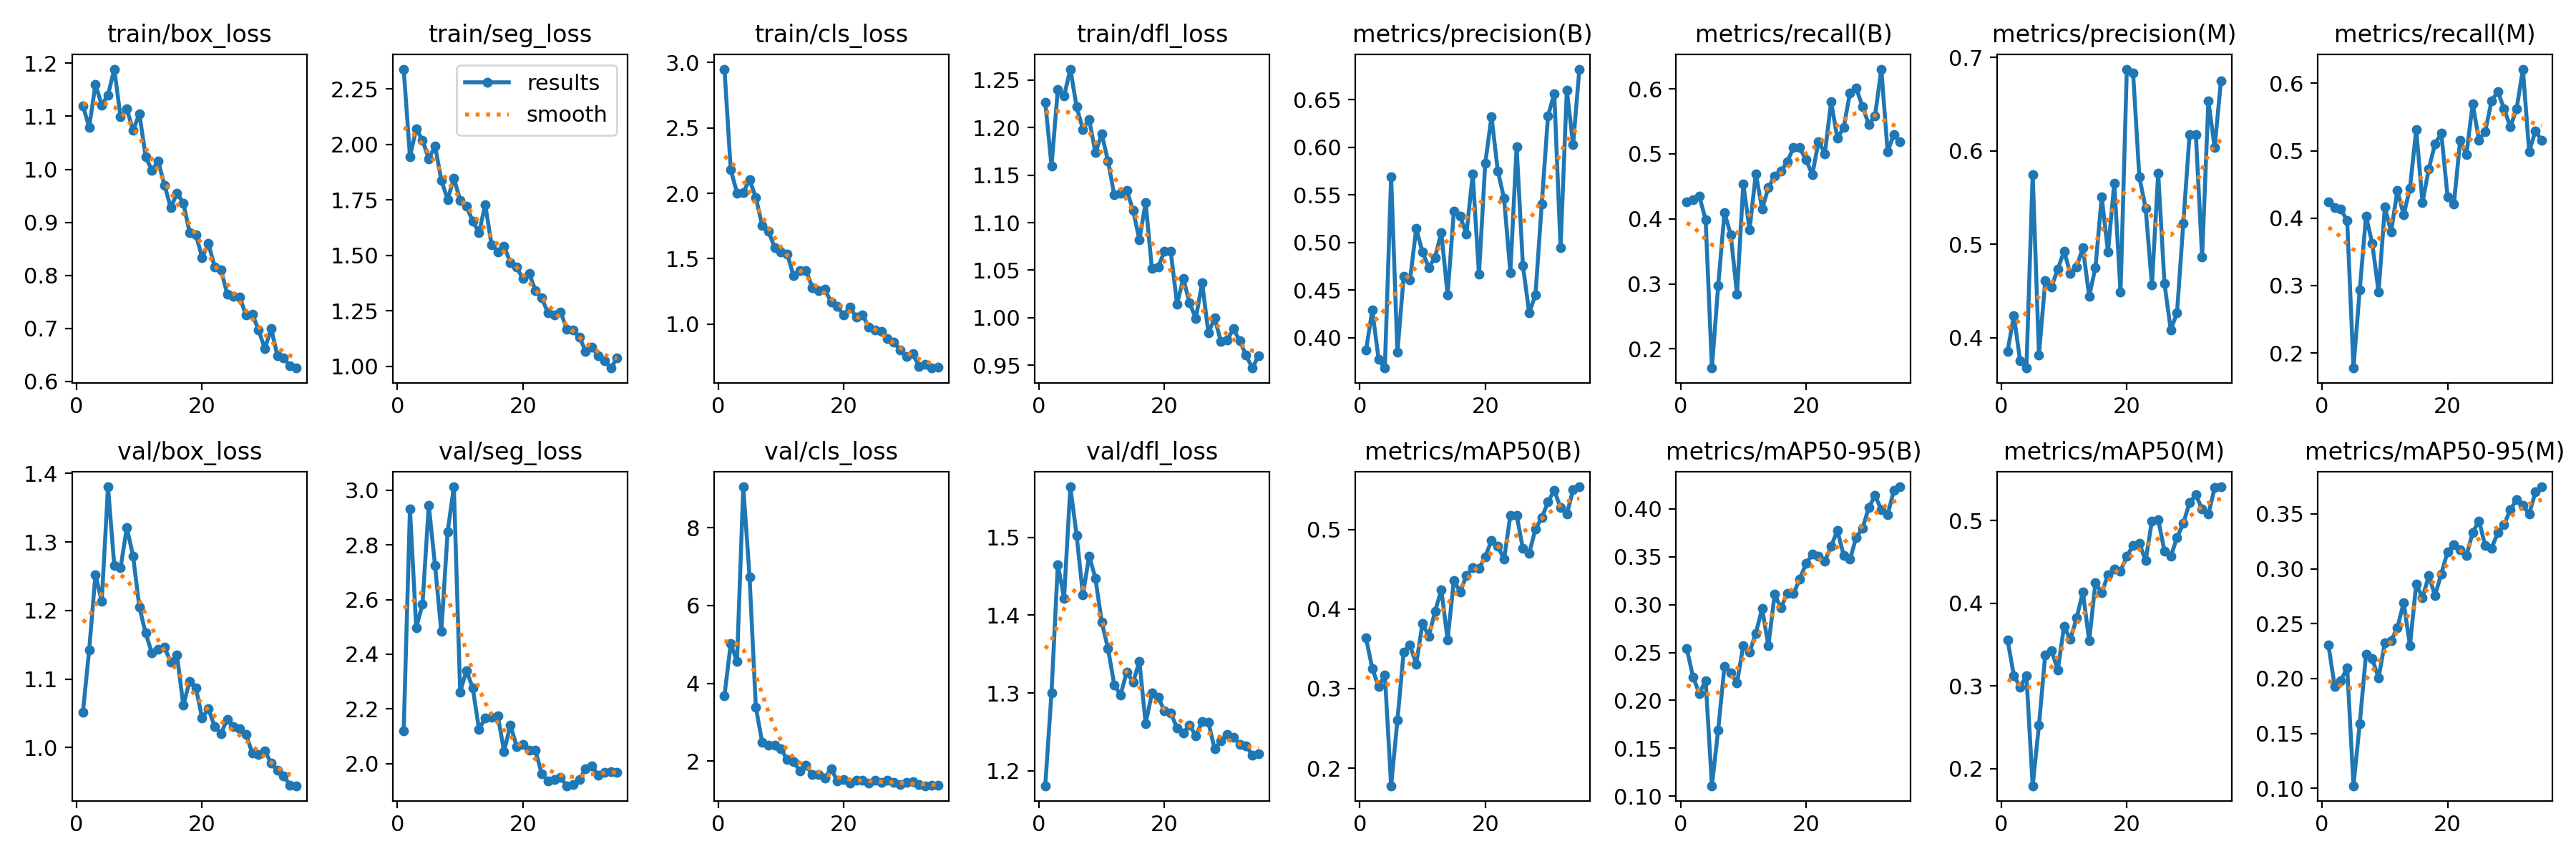
\includegraphics[width=1\linewidth]{imgs/results.png}
    \caption{Изменение ключевых метрик в процессе обучения.}
    \label{fig:metrics}
\end{figure}
\vspace{-0.5cm}

Также, была построена нормализованная матрица ошибок для определения точности предсказания необходимых классов на валидационной выборке, которая представлена на рис.~\ref{fig:confusion}.

\begin{figure}[H]
    \centering
    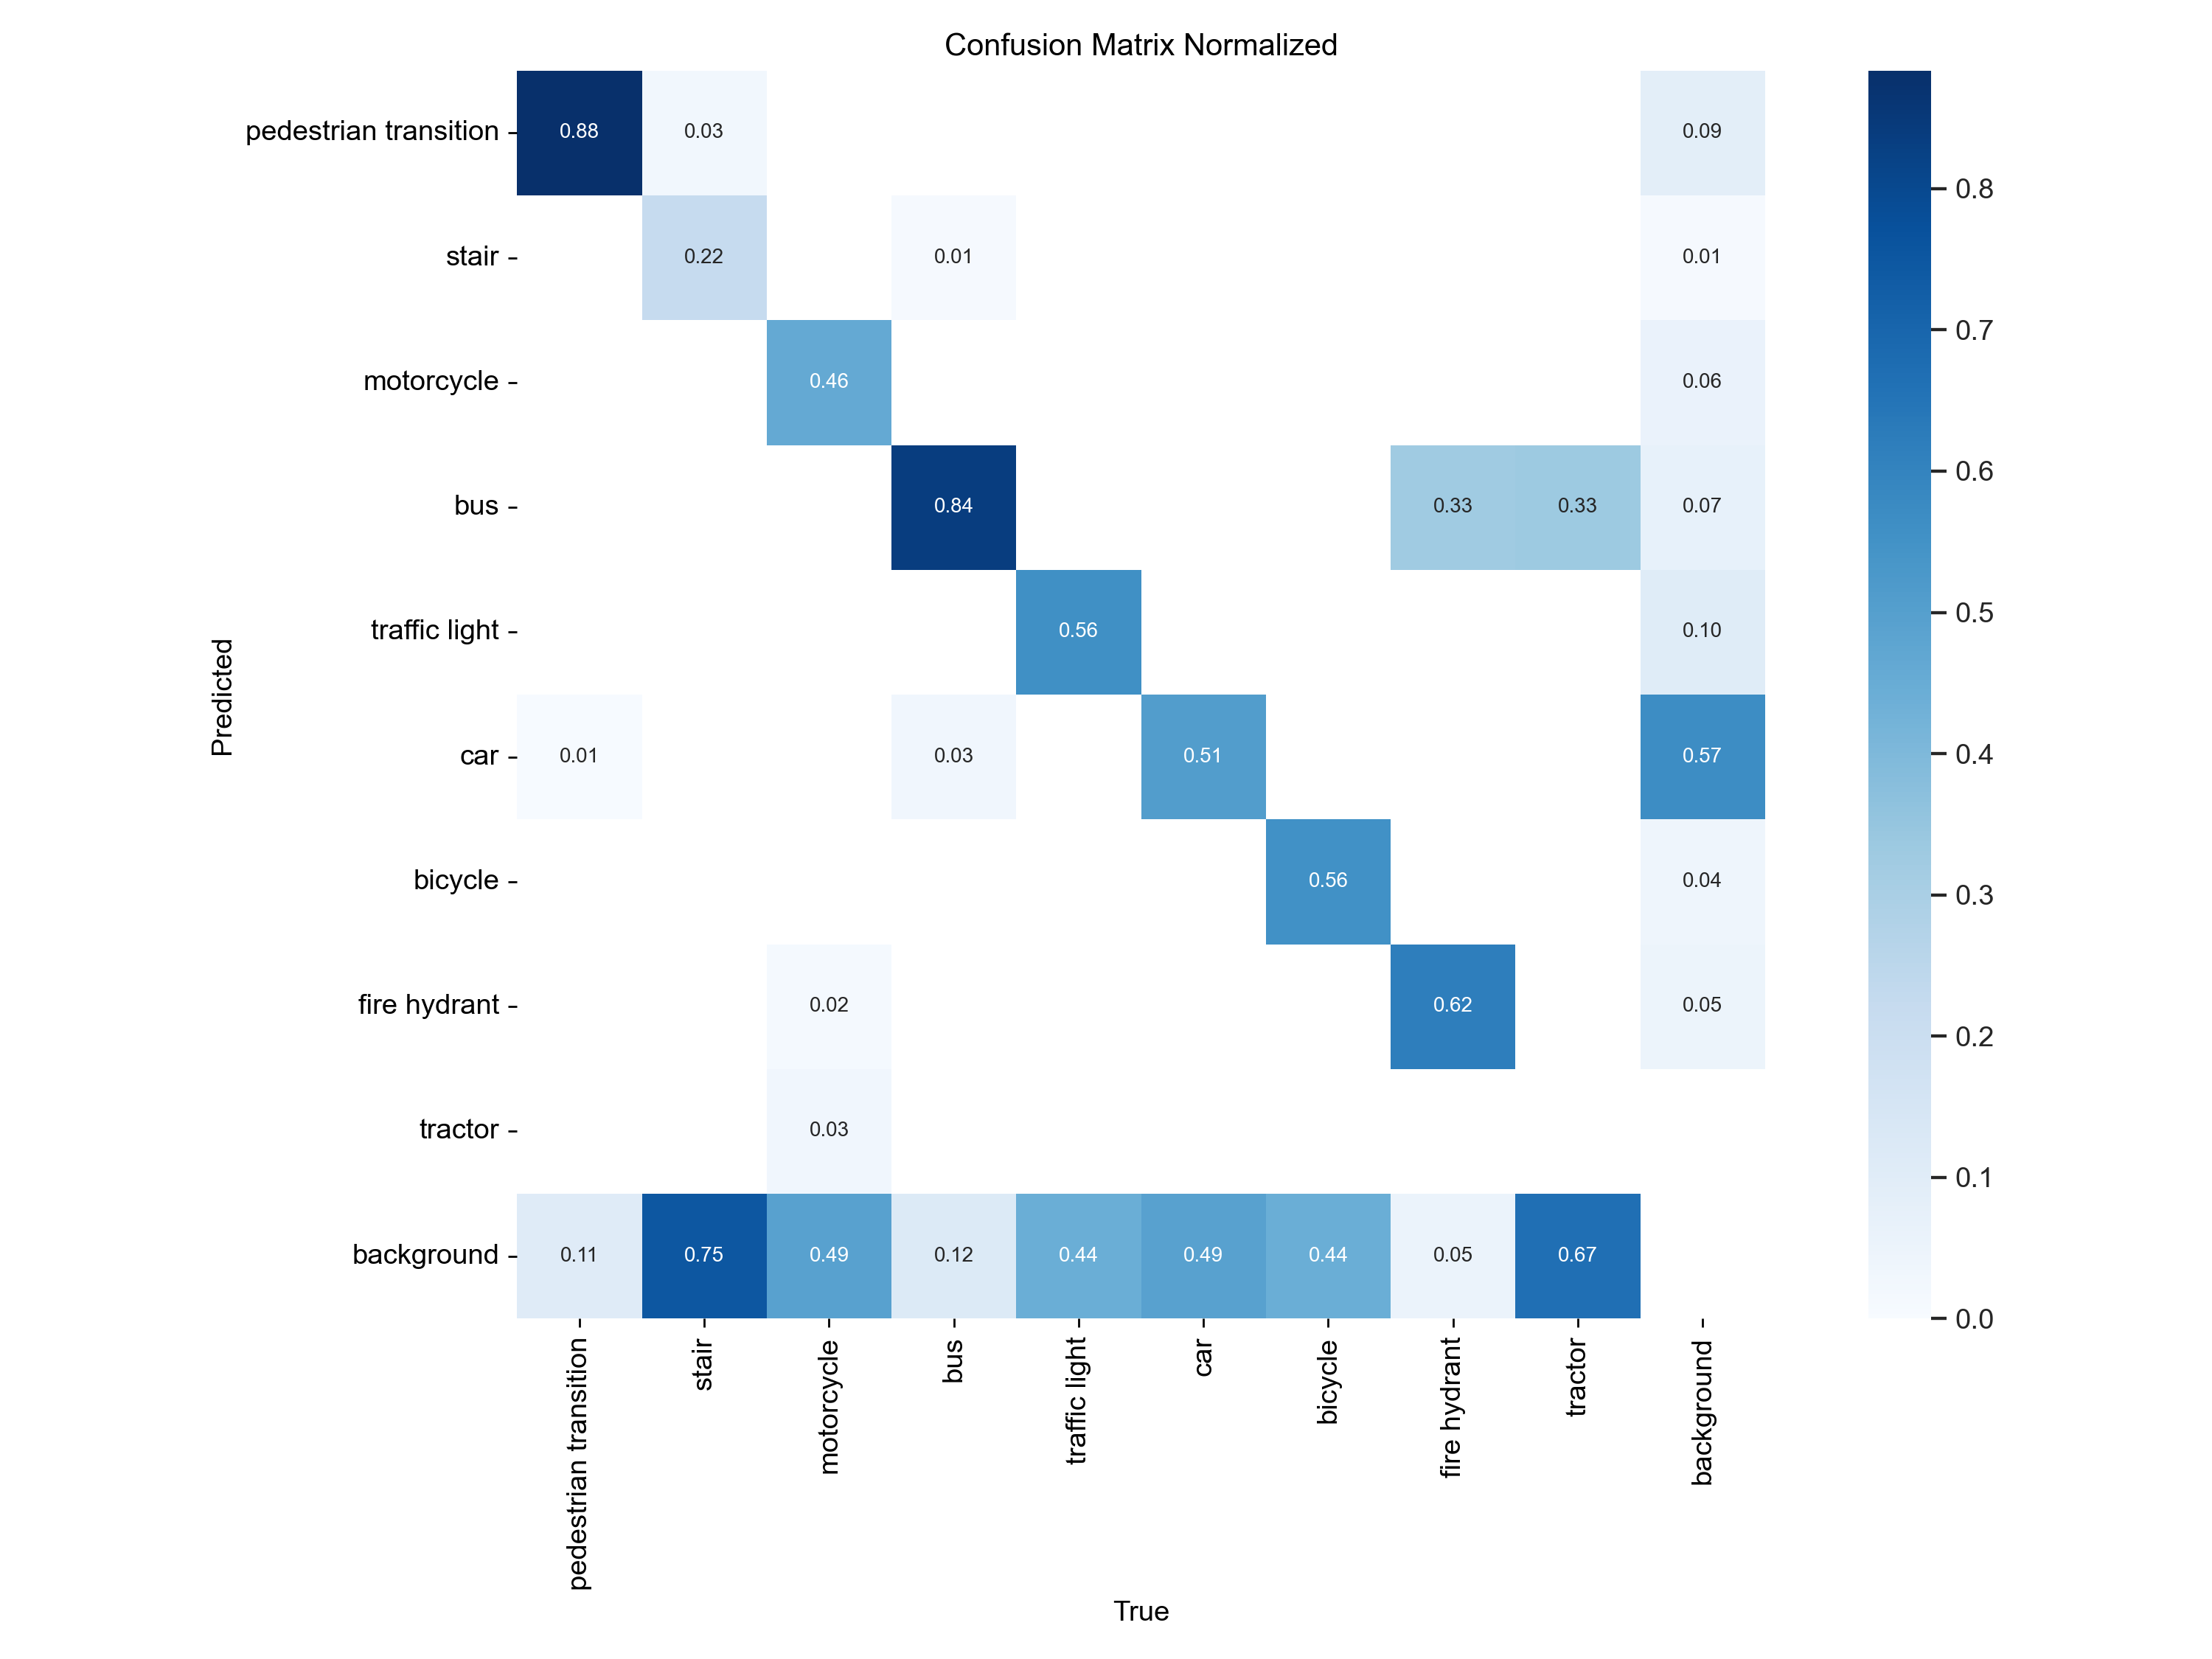
\includegraphics[width=1\linewidth]{imgs/confusion_matrix_normalized.png}
    \caption{Матрица ошибок для изображений валидационной выборки.}
    \label{fig:confusion}
\end{figure}
\vspace{-0.5cm}

\section{Тестирование модели}

После завершения обучения модель была протестирована на реальных CAPTCHA, собранных с помощью автоматического парсера, реализованного на базе библиотеки Selenium. Тестирование проводилось в автоматическом режиме, имитируя реальные действия пользователя в браузере, что позволило оценить работоспособность системы в условиях, приближенных к реальной эксплуатации.

Сценарий тестирования предусматривал выполнение следующих шагов:

\begin{enumerate}
    \item автоматический переход к странице с CAPTCHA и активация чекбокса <<Я не робот>>;
    \item извлечение изображения CAPTCHA (включая структуру сетки и текст задания);
    \item определение целевого объекта из текста задания (например, «выберите все изображения с автобусами»);
    \item разбиение изображения CAPTCHA на ячейки (в зависимости от размера сетки — 3×3 или 4×4);
    \item применение обученной модели для сегментации и классификации каждого изображения или фрагмента;
    \item определение ячеек, содержащих нужный класс, и программная симуляция кликов по ним;
    \item повторная попытка прохождения CAPTCHA в случае, если результат оказался некорректным (что также фиксировалось в логах).
\end{enumerate}

Тестирование было организовано в виде цикла, позволяющего автоматически проходить CAPTCHA до тех пор, пока не будет достигнут положительный результат. Это позволило зафиксировать частоту ошибок модели и определить случаи, в которых требуются дообучение или оптимизация.

Рабочий процесс тестирования и взаимодействия модели с CAPTCHA представлен на блок-схеме ниже.

\begin{figure}[H]
    \centering
    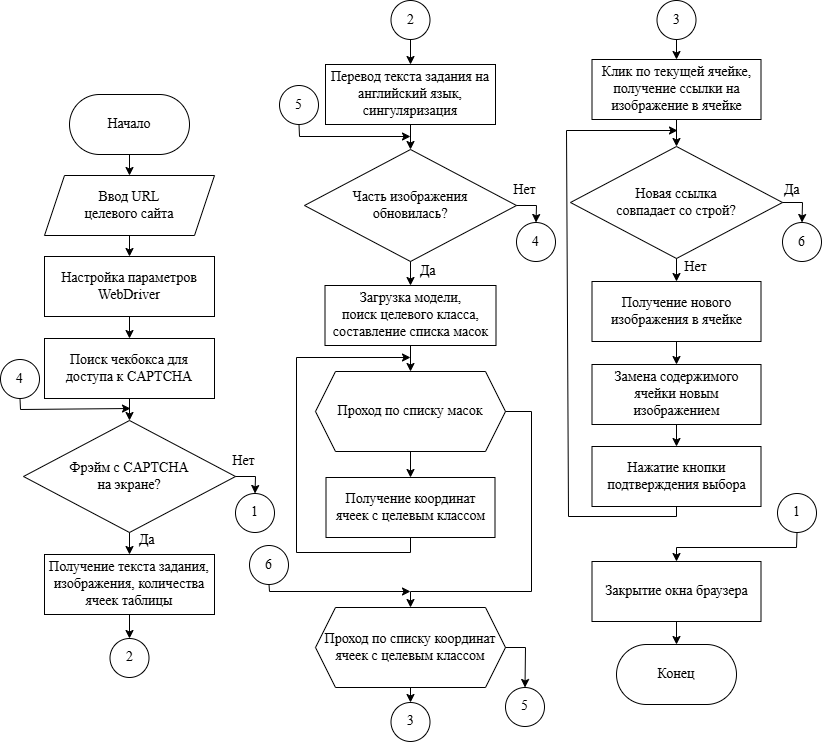
\includegraphics[width=1\textwidth]{imgs/solve_captcha_flow.png}
    \caption{Блок-схема процесса прохождения CAPTCHA.}
    \label{fig:solve-captcha}
\end{figure}
\vspace{-0.5cm}

Полученные данные используются для последующего анализа качества модели и корректировки процесса обучения. Основное внимание при анализе будет уделено типам ошибок, сложности распознаваемых объектов и влиянию качества исходного изображения на точность сегментации.
